
\chapter{The Data-Centric Approach}\label{ch:datacentric}

\section{An Opportunity Arises}

\unedit{

    Our core vision is to combine the code mobility of RPC with the flexibility offered by
    DSM-like models in a global address space with global references as a first-class abstraction. By
    imbuing data with fundamental identity and pushing an understanding of data references into the OS
    and the network, we can leverage aspects of content-based networks to reduce the coordination
    typically required in a shared, distributed address space. The programmer is then free to express
    their computation through references to code to run on some \emph{references} to data, instead
    of needing to serialize and copy \emph{values} for arguments.
    Today, developers are often forced to implement functionality such as caching, prefetching, and
    manual data movement in preparation for some operation.
    With data references as a common
    language between the OS, the network, and applications, we can move this infrastructure-level functionality
    out of the application and back \emph{into the infrastructure} where it belongs.
}

\section{A Common Language}



\unedit{
    We cannot store virtual addresses in persistent data, so we need a new way to name a word of
    persistent memory: a \emph{persistent pointer}. The persistent pointer encodes a persistent
    identification
    of data (\S~\ref{sec:invariant_pointers}) instead of an ephemeral address,
    allowing any thread to access the desired word of memory regardless of
    address space.
    This approach dramatically improves programmability, as programmers
    need not worry about the complexity of referring to persistent data with ephemeral constructs,
    improving data sharing between programs and across runs of a program. \Twizzler still makes use of virtual
    memory \emph{hardware} to provide isolation and translation, but persistent data
    structures should not be written in terms of virtual addresses.


    \paragraph{The Death of the Process.}
    Processes as a first class OS abstraction are, like virtual addresses, unnecessary; a traditional process couples
    threads of control to a virtual address space, a security role, and kernel state.
    %an environment for a set of threads to operate in.
    However, with the kernel removed from
    persistent data access, much of that kernel state (\eg file descriptors) is unnecessary,
    leading to a decoupling of mechanisms:
    nothing fundamentally connects a virtual address space
    (a piece of ephemeral context used to access data) and a security context (\emph{what} data
    threads may access).
    Instead, a data-centric OS can keep the good parts of a process but \emph{separate} virtual address
    translation and security roles, allowing threads to select one of each as needed.


    %\footnote{Of course, we do not want to throw out \emph{good} parts of a process. Mechanisms like
    %protection, shared memory, and (in some cases) hierarchical responsibility still have their uses,
    %but do not need to be coalesced into a single, rigid abstraction. Their separation would have
    %significant effects on the POSIX model, but our model, but our model, built from clean abstractions,
    %can make use of gained flexibility (as we will see in \S~\ref{sec:eval}).}.


    % maybe move this to 4.3?
    The process abstraction is just one example. Persistent data access plays a key role in OS
    abstraction design, and we need to avoid complexity arising from combining old and new interfaces.
    Hence, we need to consider the
    wide-reaching effects of changing the persistence model on \emph{all} aspects of the system, not
    just I/O interfaces. \NVM gives us an opportunity to design an OS around the requirements
    of the target programming model instead of trying to mold support libraries around existing
    interfaces. While it is important that we provide support for legacy applications,
    it is these applications that should be relegated to support libraries; new applications built for
    the programming model should get first-class OS support.
}

\unedit{
    \subsection{Computation and References}

    First-class support for call-by-reference instead of by-value allows an invoker to refer to data that \emph{they
        do not have locally}. This allows greater freedom in the interface design between decoupled components.
    Figure~\ref{fig:rpccopy} shows possible solutions to a problem like the
    example in Section~\ref{sec:example}, wherein an operation is scheduled to run on Carol using data
    currently located on Bob. Part (1) shows the na\"ive approach where the invoker copies the data
    locally (step i) before forwarding it to Carol (step ii) and eventually invoking the intended computation
    (step iii).  In an attempt to alleviate an unnecessary copy, we could implement an additional
    RPC on Carol that allows it to copy data over from Bob itself (steps i and ii in part (2)) before we
    finally invoke our computation. Both (1) and (2) require additional logic on Alice
    to work---the programmer had to perform the infrastructure level task of data
    movement.  Fundamentally, these issues arise because the system's core abstraction is
    location-based---the programmer is forced to manually orchestrate machines or resort to
    costly copying.

    Figure~\ref{fig:rpccopy} part (3) is closer to our vision. The first step is for
    the computation to move to Carol instead of first moving data in preparation.  This may seem like a
    minor point, but it is not---by specifying \emph{up-front} the computation we want to perform, we
    open the door for lower-level optimization to examine our requests before we go around manually
    moving data.  In fact, in our model the programmer would not be directly asking Carol to perform the
    computation; instead the placement decision would be made by the system. Once the code starts
    executing, we can then move data on demand instead of having to move the entire
    object.  Of course, the implementation is significant---without a global address space like
    the one we are proposing, implementing (3) would require brittle code that either tightly couples
    Carol and Bob or forces Alice to participate in the data movement by asking it to provide a
    location-based reference to the data on Bob\footnote{Aside from the complexity, this also
        opens up TOCTTOU errors.}.


    \begin{figure}
        \centering
        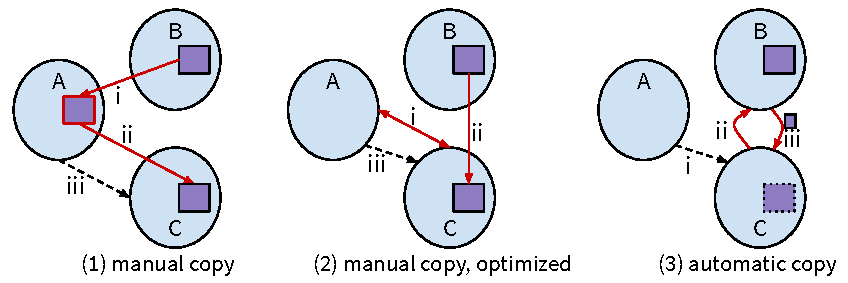
\includegraphics[width=\linewidth]{fig/copy}
        \caption{Rendezvous of data and compute. Solid red arrows are additional
            infrastructure-level tasks that are not fundamental to the requested computation.}
        \label{fig:rpccopy}
    \end{figure}

    As discussed previously, the ``good'' use case of RPC is one where code and data
    co-location has already been preordained by initial decoupling (after which it is rigid) and
    data transfer is minimal---often manifesting as something like a fronted key-value store service. This restricts
    code mobility (as it accounts for no change to decoupling later), and requires a myriad of RPC calls
    to implement all the ways a programmer might wish to view data (one need only look at the many S3
    APIs available as an example).
    If we limit ourselves to traditional RPC, any situation (such as the one discussed in
    Section~\ref{sec:example}) that does not fit this pattern either results in expensive data movement
    and complex application logic, or it must be dismissed altogether and the application redesigned.
    By allowing applications to pass data references instead of just values, and by making data
    references a first-class abstraction in the OS and the network, applications become much simpler to
    express efficiently, even for what would be considered pathological cases for RPC.

    \paragraph*{Serialization.}
    %
    In traditional host- and process-centric systems, virtual memory spaces are private to a
    program instance and thus addresses are too. As a result, we serialize any data that passes between
    hosts (and sometimes even processes) because memory addresses on one host do not translate to any
    other host. However, in our model, pointers refer to data within the \emph{global} address space,
    and thus a data structure containing pointers can be copied from one host to another with merely a
    byte-level copy, alleviating 100\% of the loading overhead discussed in Section~\ref{sec:example}
    and leaving only data transfer costs, which are fundamental. These transfer costs, however, can now
    be included in cost-models when making placement decisions more easily, as they do not need to take
    the additional loading time into account.

}


\section{The Design Space}



\unedit{
    % maybe this goes in into or 4.1?
    Operating systems provide abstractions for data access that reflect the hardware for which
    they were designed. Current I/O interfaces and abstractions reflect the structure of mutually
    exclusive volatile and persistent domains, the hallmarks of which are heavy kernel involvement for
    persisting data, a
    need for data serialization, and complexity in data sharing requiring the overhead of
    pipes or the management cost of shared virtual memory. However, the introduction of low latency and directly
    attached
    \NVM into the memory hierarchy requires that we rethink key assumptions such as
    the use of virtual addresses, the kernel's involvement in persistent I/O, and the way that
    programs operate on and share persistent data~\cite{faraboschi:hotos15}.
}


\unedit{
    These characteristics imply two basic requirements for OSes
    to most effectively use \NVM:
    \begin{enumerate}
        \item[(R1)] \textbf{Remove the kernel from the persistence path.}
            This addresses both
            characteristics. System calls to persist data are costly; we must provide
            lightweight, direct, memory-style access for programs to operate on persistent data.
        \item[(R2)] \textbf{Design for pointers that last forever.}
            %This is a direct
            %consequence of applications using in-memory data structures in persistent memory.
            Long-lived data structures can directly reference persistent data, so
            pointers must have the same lifetime as the data they point to.
            Virtual memory mappings are, by contrast,
            ephemeral and so cannot effectively name persistent data.
            Persistent data is, by definition, accessed by multiple actors, both
            simultaneously and over time, and thus must be stored in a form that is conducive to sharing without
            needing the ephemeral context associated with a particular actor.
    \end{enumerate}
}


\unedit{
    We call an OS that meets both requirements R1 and R2
    \emph{data-centric}, as opposed to current OSes, which are \emph{process-centric}.
    Operations on persistent, in-memory data structures are the primary functions of a data-centric OS,
    which tries to avoid interposing on such operations, preferring instead to intervene only when
    necessary to ensure properties such as security and isolation. To meet both of these requirements
    a data-centric OS must provide effective abstractions for identifying data independent
    of data location, constructing persistent data relationships that do not depend on ephemeral
    context, and facilitating sharing and protection of persistent data.
}


\unedit{

    While considering a single machine as a distributed system\footnote{While the system is
        distributed, and contains communicating entities, it is not \emph{truly} a traditional
        distributed system, since a single machine does not include partial-failure semantics (and the
        cases where it does are rare enough that they may be largely ignored); often a partial failure
        of a component is instantly upgrade to total failure. However, the messaging semantics of
        distributed systems are present.} has been examined from the
    perspective of OS design~\cite{baumann:sosp09}, the extent to which we are proposing has not been.
    \emph{Each} device, including CPU sockets, acts like a component containing a local memory with
    \emph{direct} access to a pool of shared, persistent storage.

    Such a model has two significant implications:
    \begin{enumerate}
        \item Protection of data within this system is of utmost importance, considering how each of
              these devices
              could run an entire operating system with application suites. The green lines in
              Figure~\ref{fig:sys_arch} represent control paths, showing how memory access is administrated. Note
              that the CPU, while similar in some respects to other devices, is distinguished in that it sets
              security policies for the system\footnote{Only in supervisor mode; user-space applications can only
                  administrate devices that have been mapped into their address spaces.}. The \emph{enforcement}
              of those policies is handled by the MMU and the IOMMU, both of which apply a mapping of virtual
              addresses to physical addresses along with access restrictions.
        \item The addresses emitted by such devices are typically physical addresses that DMA engines
              operate on. However, similar to \observation~\ref{hetero-mem} above, emitting physical
              addresses has significant complications in our model, necessitating the need for hardware to
              abstract physical memory into an object-space as well. Current systems can implement this
              (along with protection) through the IOMMU for hardware devices and MMU for the CPU.
    \end{enumerate}

    These implications combined with \observation~\ref{hetero-mem} leads to another point:

    \observe{sls}{The CPU and devices must agree on a single, global abstracted view of
        shared physical memory, leading to a system-wide single-level store interface (shown in
        Figure~\ref{fig:log_sys_arch}). Protection is
        enforced by hardware devices such as the IOMMU, and devices can operate on data objects as
        opposed to physical memory directly.}

    In the case of specialized hardware running programs, this grants hardware better access to global
    memory because it does not need to coordinate and the system can trust it more (since the IOMMU can
    enforce security). For simple I/O controllers, like an NVMe device, it allows programming of such
    devices in a more efficient and simpler way---instead of translating object pages into physical
    addresses, it can issue DMA requests directly to object pages instead.


    \begin{figure}
        \centering
        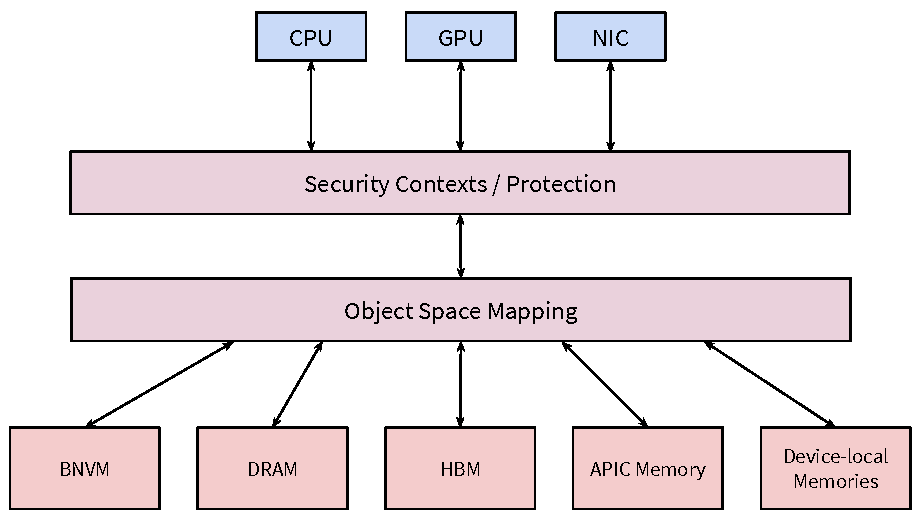
\includegraphics[width=\linewidth]{fig/log_sys_arch}
        \caption{Logical view of the system architecture. Mapping hardware such as the IOMMU would allow
            \emph{all} devices to see a single-level store instead of raw physical memory.}
        \label{fig:log_sys_arch}
    \end{figure}


    An example of this would be if a NIC is processing data it received in a packet, and that data
    references data in another data object. If there were no abstraction layer, the NIC would need to
    either interrupt the CPU to ask where the data is, or it would need to keep a map of objects in
    physical memory itself. The latter adds to management costs of maintaining such maps for all
    hardware devices in the system when data placement changes, and the former results in performance
    degradation (due to interrupting the CPU) and requires additional management code to assist in
    making data transfers on behalf of the hardware devices\footnote{Many current devices today will
        still need this. However, we are planning for a system model in which it is less necessary. Many
        devices today fit this model, including some GPUs and special off-chip processing
        accelerators.}. This also leads to another \observation about data movement, since data
    processing decisions will need be made by devices autonomously:

    \observe{mem-to-mem}{Operating systems will need to provide a way for applications to specify data
        movement in a system declaratively, so that data movement decisions can be made largely without user
        involvement.}

    %A natural consequence of such a distributed system is heterogeneous computing, where we have
    %different types of processors accessing memory simultaneously. This could be as simple as an x86
    %processor and an ARM processor both operating on shared memory, where the system offloads
    %computationally nonintensive tasks to the ARM chip, but also encompasses our system design above.
    %For example, ARM GPUs can (and do) access global memory with cache coherence with the CPU (CITE).
    %The jury is still out on scaling-up cache coherence in this way, and systems will need to support
    %both devices that operate on only local memory and devices which operate on shared memory.



    The system design shown in
    Figure~\ref{fig:sys_arch} is not necessarily the end evolution of treating a single machine as a
    distributed system of components. We could imagine treating the CPU like any other component which
    accesses shared memory through a controller that itself enforces memory protections and mappings.
    However, such a model is easier to reach and program for as an evolution of our proposed system
    design presented here. Furthermore, Figure~\ref{fig:sys_arch} shows a system design that can be
    realized \emph{now}, allowing us to construct a real system to explore our goals.


}


\subsection{Hardware Versus Software}

\unedit{
    The challenges introduced by BNVM in mapping virtual addresses to physical
    addresses are the different lifetimes of data with respect to
    the references to that data and the heterogeneity of physical memory. Software and hardware have
    different requirements for this mapping, in the following respects:

    \begin{enumerate}
        \item[Latency.] Prior persistent data access schemes relied on system calls to
            operate on persistent storage. BNVM's low-latency can no longer tolerate the cost of those
            system calls. Instead, programs must have direct access to
            persistent data via load/store instructions. Similarly, hardware must be able to
            transfer data to and from BNVM using DMA.
        \item[In-memory data structures.] Direct access to persistent memory removes the loading and
            unloading cost, but we must \emph{also} remove the cost of data serialization: since
            persistent data is located in-memory, programs can operate on data as in-memory data
            structures using standard programming techniques. This change
            is not an issue for hardware, which treats data as a ``bag of bits''.
        \item[Data lifetime.] If persistent data is stored as in-memory data structures, then
            applications need a way to refer to data such that references have the same lifetime
            as the referenced data, a requirement that fundamentally arises from the need for
            to construct references that encode the relationships between data. Applications can store
            \emph{persistent pointers} that encode a more persistent name for data than an ephemeral
            virtual address.
            Again, hardware has no such requirement, since it neither constructs
            nor interprets relationships between data. Devices that need to consider data
            relationships do so in software running atop the hardware.
        \item[Mappings.] Both software and hardware must have a way of translating a
            %$\langle \mathit{object}, \mathit{offset} \rangle$ reference
            persistent pointer into a physical address.
            This mapping may change frequently as the OS changes allocation of physical
            pages to data (\eg, to persist a piece of data).
            %to objects, potentially moving objects in and out of BNVM (\eg, to persist an object).
            Hardware need only know
            %the mappings for a short time, and need not even know the ``canonical''
            %name for the object---
            %it simply needs to know
            how to access data in memory
            for a single operation. In contrast, software must have longer-term mappings, and must
            be able to support data shared between threads, potentially mapped into the threads
            in different places.
        \item[Memory heterogeneity.] Hardware and the operating system must know about different
            types of memory, \eg DRAM and BNVM.
            Software need only know how to allocate
            from the different types, and should not deal with other differences. Hardware, however,
            will need to know when data is moved between memory types if it wishes to correctly emit loads and stores
            requested by software.
    \end{enumerate}

    Our design must support appropriate abstractions for both software and hardware, facilitating the
    use of \emph{persistent pointers} to long-lived data for applications while providing hardware and
    the OS with the ability to move data in, out of, and around physical memory, preferably only using
    existing hardware functionality. We first abstract memory into \emph{objects},
    where related data with similar access semantics (\eg, an entire B-tree, where all nodes are subject
    to the same access control, \emph{etc}.) are placed in a single object and identified by
    a \emph{globally} unique ID. IDs are formed via hashing, partitioned allocation, or other methods that prevent collisions
    of IDs across machines with high probability.
    %A programmer could, for example, place an entire B-tree within an object (as the
    %tree itself has similar access control, etc.).
    %, or create a tree that spans multiple objects with
    %pointers between them.

    We propose two abstractions to provide effective access to objects for both hardware and software:
    a \emph{global object space}, which facilitates persistent pointers (discussed below), and a
    \emph{logical object space}, which allows hardware to address data without needing knowledge of the
    data's physical location. We split these abstractions and consider them different because of the
    different requirements discussed above; software must worry about reference lifetime, whereas
    hardware's access to objects is disconnected from persistence. On the other hand, today's hardware
    must worry about physical location of data, which (with BNVM) is now more
    likely to change over time.
}

\unedit {
    \paragraph{Hardware and Memory}

    The interface presented to hardware must enable interaction with a
    \textit{heterogeneous memory system} and support the abstraction of an object space rather than a
    collection of flat memory spaces. Unlike applications, hardware has no need for
    creating long-lived pointers to locations within objects. Rather, hardware must
    have the ability to transfer large chunks of objects to, from, and around memory, and must be able to
    manage different \emph{types} of memory, preferably in a way that is largely transparent to
    applications.

    Requiring hardware to access a global object space through a $\langle \mathit{object},
        \mathit{offset} \rangle$ tuple is unnecessary overhead and complexity---hardware need only ever
    access the ``working set'' of objects currently undergoing computation. Thus, our design abstracts
    the view from hardware of physical memory into a \emph{logical object space}, an address space that
    maps contiguous objects within it to physical memory pages, managed by the
    operating system. This solves the heterogeneity problem by allowing hardware to refer to data within
    objects instead of physical addresses, whose lifetimes are much smaller than the objects, and
    doesn't require hardware to emit (likely large) addresses for the global address space.

    While SASOSes are not a viable solution to the problem of persistent pointers, they are
    \emph{a} solution to implementing the logical object space.  Hardware, and the CPU, are
    directly connected, reducing the cost of invalidation and coordination of an address space.
    Additionally, this address space is \emph{intermediate} and hidden from programs---a virtual
    address is translated to the logical object space, after which the address is translated to a
    physical location (shown in Figure~\ref{fig:twolevel}). This translation for
    applications (after the virtual address translation) and that of hardware is the same, reducing the
    management complexity for the OS, discussed in Section~\ref{sec:os:addrspace}.

}


\subsection{Twizzler: A Point in This Space}


\unedit{
    The consequences of meeting the requirements of these hardware trends
    %and the consequences of those requirements
    define a bounded design space for data-centric OSes. We have
    chosen a point in that space and built \Twizzler, our approach to providing
    applications with efficient and effective access to \NVM. In the
    following section we will discuss how our four primary abstractions---a low level persistent object
    model, a persistent pointer design, an address space mechanism called \emph{views}, and a
    security context mechanism---achieve these goals of removing the kernel from the persistent data
    access path.
}


\unedit {
    There are several design principles that we believe a successful system must adhere to:
    \begin{enumerate}
        \item \textbf{Get the OS out of the way}
              Addressing \observation~\ref{os-out-of-the-way} requires removing kernel invocations from the
              common path of persistent data access. Instead, we provide applications with methods for
              accessing persistent data directly as in-memory data structures, thereby removing the
              overhead of kernel boundary crossings. Note that this necessarily implies a shared-memory
              style interprocess communication. When shared memory is not possible, however, the system
              must support some form of message passing.

              Such a model also addresses \observations~\ref{data-movement} and~\ref{mem-to-mem}, since
              by removing the kernel from the path of persistent, shared data access, hardware can more
              autonomously operate on data objects.

        \item \textbf{Orthogonal persistence} The emergence of BNVM will make persistence the norm
              rather than the exception, and so the programming model should have both \emph{persistence
                  by default} and \emph{transparent, implicit} persistence. However, in accordance with
              \observation~\ref{consistency}, applications will need to play a significant role in
              consistency of persistent data.

        \item \textbf{Single address space} We will provide a single address space of data objects to
              applications \emph{and hardware} called the \emph{object-space}. This addresses
              \observations~\ref{hetero-mem} and~\ref{sls} by abstracting
              different types of physical memory and allowing DMA transfers to refer to data within
              objects instead of physical addresses. Applications running on the CPU will, too, see this
              same address space, allowing references to more easily pass around the system. Additional
              benefits include:
              \begin{enumerate}
                  \item Allows devices to refer to object data without needing to be aware of where the
                        object is physically located. This is advantageous in a heterogeneous memory
                        hierarchy, since data may move often.
                  \item Simplified security policy: security policy can be defined for objects instead of
                        physical address.
                  \item More autonomous operation of devices: if the system can rely on security
                        enforcement via the IOMMU, these devices can securely access data in main-memory on
                        their own without needing to be reprogrammed often.
                  \item Simplified system programming: the unified data access model of Twizzler allows
                        programmers to write programs that operate on data
                        that can then run on any device, from the CPU to a NIC, without needing to
                        specialize their application.
              \end{enumerate}
              Of course, if a device (CPU or otherwise) wishes to provide additional layers of abstraction
              (such as segmentation or virtual address spaces) atop this single address space to ease
              programming, they may do so (to assist in addressing \observation~\ref{sasos}). Internally, however, the object-space allows hardware devices
              to agree on a way to reference that data within the system, regardless of where it may be
              physically located.
        \item \textbf{Data movement and security} should be handled declaratively, so as to not require invoking
              the CPU whenever such a decision needs to be made (\observation~\ref{mem-to-mem}).
    \end{enumerate}
}

\unedit{

    \Twizzler is a stand-alone kernel and userspace runtime that provides execution support
    for programs. It provides, as first-class abstractions, a notion of threads, address spaces,
    persistent objects, and security contexts. A program
    typically executes as a number of threads in a single address space (providing backwards
    compatibility with existing programming models), into which persistent objects are mapped on-demand.
    Instead of providing a process abstraction, \Twizzler provides \emph{views}
    (\S~\ref{sec:view}) of the object space, which formalizes the notion of ephemeral context within our
    model by allowing programs to map objects for access,
    and \emph{security contexts} (\S~\ref{sec:sec}) which define a thread's access rights to objects in the system.
    \Twizzler provides persistent pointers  (\S~\ref{sec:invariant_pointers}) for
    programs, as well as primitives to ensure crash-consistency
    (\S~\ref{sec:crash}). The thread abstraction is similar to modern OSes; the
    kernel provides scheduling, synchronization, and management primitives.
    Figure~\ref{fig:twz_sys_overview} shows an overview of the system
    organization and how different parts of the system operate on data objects.

    \begin{SCfigure}[b]
        \centering
        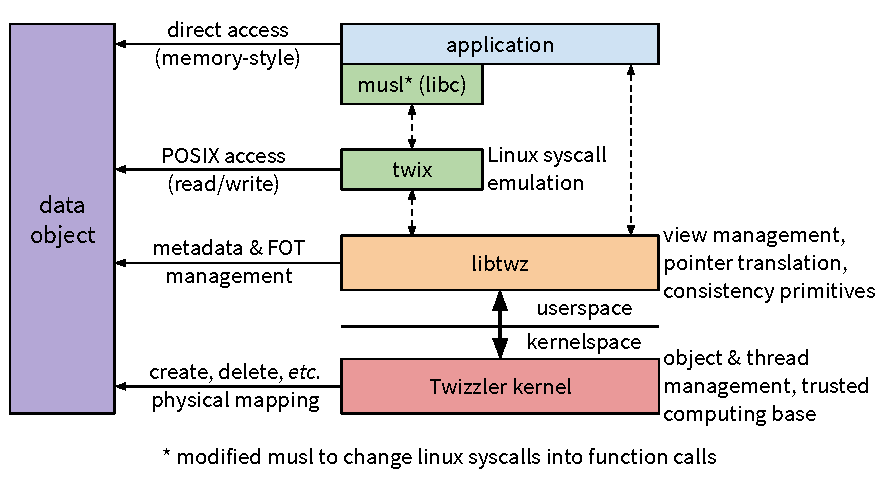
\includegraphics[width=\linewidth]{fig/sys_diag}
        \caption{\Twizzler system overview. Applications link to \texttt{musl} (a C library),
            \texttt{twix} (our Linux syscall emulation library), and \texttt{libtwz} (our standard
            library). Through \texttt{musl}, they may act on persistent data with POSIX interfaces,
            though we expect \Twizzler applications to operate directly on persistent data with
            memory-style semantics.}
        %They can directly access objects or they can use legacy POSIX methods.}
        %The \texttt{libtwz} library provides library-OS functionality and manages the
        %address space and kernel interaction. The kernel manages objects, schedules threads, and
        %enforces security by programming MMU hardware.}
        \label{fig:twz_sys_overview}
    \end{SCfigure}


    \Twizzler's kernel acts much like an
    Exokernel~\cite{Kaashoek,engler:sosp95}, providing sufficient services for a
    userspace library OS, called \emph{\libcore}, to provide an execution environment for applications.
    The primary job of \libcore is to manage mappings of persistent objects into the address space (\S~\ref{sec:view})
    and deal with persistent pointers (\S~\ref{sec:invariant_pointers}).
    \Twizzler also exposes a standard library that
    provides higher level interfaces beyond raw access to memory. For example, software that better fits
    message-passing semantics can use library routines that implement message-passing atop shared
    memory. \Twizzler's standard library provides additional
    higher level interfaces, including streams, logging, event notification, and many
    others. Applications use these to easily build composable tools and pipelines for
    operating on in-memory data structures without the performance loss and complexity of explicit I/O\@.

}

\section{A Historical Look}


\unedit{\label{sec:relwork}

    %The introduction of byte-addressable non-volatile memory presents an outstanding
    %opportunity to rethink the way that OS's handle memory and storage.

    % Working with new technologies often allows past, merely theoretical ideas a
    % chance to be practical.

    \Twizzler's design
    is shaped by fundamental OS
    research~\cite{corbato_introduction_1965,chase:tocs94,k42,engler:sosp95,Kaashoek,engler1995avm,engler1995exterminate},
    which,
    while approaching similar topics described in
    Section~\ref{sec:datacentric}, often did not consider \emph{both} design
    requirements simultaneously, resulting in an incomplete picture for \NVM.
    Recent research on building \NVM data structures~\cite{volos:asplos11,coburn:asplos11,condit:sosp09,debnath:vldb10,lu:tos16,hu:atc17},
    often focuses on building data structures that
    provide failure atomicity and consistency.
    In contrast, we explore how \NVM affects programming models while potentially improving performance.
    We draw from recent work on providing OS support for \NVM systems~\cite{caulfield:micro10} and work
    providing recommendations for \NVM systems~\cite{mehra:ipdps04}, integrating
    object-oriented techniques and simplified kernel design
    to provide high-performance OS support for applications running on a single-level
    store~\cite{shapiro:sosp99,bailey:hotos11}.

    % Our approach will leverage non-volatile memory characteristics to greatly
    % reduce the need for an OS stack and provide full system
    % resumability.
    %, we draw on prior object-oriented OS design work to
    %simplify the kernel using techniques developed in systems such as K42~\cite{k42}
    %and
    %Exokernel~\cite{kaashoek_application_1997, engler:sosp95}.

    %\subsection{Memory Model}
    \paragraph{Memory and Object Model}

    Multics was one of the first systems to use segments to partition memory and
    support relocation~\cite{bensoussan:sosp69,daley:cacm68}. It used segments to
    support location independence, but still stored them in a file system, requiring manual linkage
    rather than the automated linkage in \Twizzler. Nonetheless, Multics demonstrated that the use of
    segmenting for memory management can be a viable approach, though its
    symbolic addresses were slow.

    The core of \Twizzler's object space design uses concepts
    from Opal~\cite{chase:tocs94}, which used a single virtual
    address space for all processes on a system, making it easier to share
    data between programs. However, Opal was a single-address space OS, which is insufficient for
    \NVM~\cite{bittman:plos19,bittman:hotstorage19},
    and, while it resulted in a speedup of data transfer and sharing as well as interfacing with
    devices, it did not address issues of file storage and name resolution. It also
    still required a file
    system, since there was no way to have a pointer refer to an object with changing identity,
    whereas our approach
    of late-binding for pointers
    removes the need for an explicit file system.  Other single-address space
    OSes, such as Mungi~\cite{heiser:scse9314},
    Nemesis~\cite{roscoe:osr94}, and Sombrero~\cite{skousen:ipccc99}, show that
    single address spaces have merit, but, like Opal, did not consider how the use
    of \NVM would alter their design choices; in particular, how the use of fixed addresses
    results in a great deal of coordination that is unnecessary in our approach.
    OSes such as HYDRA~\cite{wulf:cacm74} provide functionality similar to cross-object pointers;
    however, in \Twizzler, we extend their use from procedures-referencing-data to
    a more general approach. Furthermore, they required
    heavy kernel involvement, an approach incompatible with
    our design goals.

    Single-level stores~\cite{shapiro:usenix02,shekita:uwtr956,dearle:cs94} remove the
    memory versus persistent storage distinction, using a single model for data
    at all levels. While well-known,
    ``little has appeared about them in the public
    literature''~\cite{shapiro:usenix02}, even since the EROS paper.
    Our work is partially inspired by Grasshopper~\cite{dearle:cs94}, AS/400, and orthogonal persistence systems,
    but while these are designed to provide an illusion of persistent
    memory, \Twizzler is built for real \NVM and focuses on providing a truly global object space with
    global references without cross-machine coordination.
    Clouds~\cite{dasgupta:computer91} implemented a distributed object store in
    which objects contained code, persistent data, and both volatile and
    persistent heaps. Our approach uses lighter-weight objects, allowing direct
    access to objects from outside, unlike Clouds. Software persistent
    memory~\cite{guerra:atc12}, designed to operate within the constraints
    of existing systems, built a persistent pointer system using explicit
    serialization without cross-object references, in contrast to \Twizzler.
    %In contrast,
    %\Twizzler develops mechanisms that leverage \NVM,
    Meza~\cite{meza:weed13}
    suggested hardware manage a hybrid persistent-volatile store with
    fine-grained movement to and from persistent storage. Since
    persistence in \Twizzler is to \NVM, we need not interpose on
    movement between storage and memory,
    instead simply managing memory mappings of persistent objects,
    reducing OS overhead.

    Recently, several projects have considered the impact of non-volatile
    memories on OS structure. Bailey,
    \etal~\cite{bailey:hotos11} suggest a single-level store design.
    Faraboschi, \etal~\cite{faraboschi:hotos15} discuss challenges and inevitable system organization
    arising from large \NVM, and we follow many of their recommendations.
    %and using
    %\NVM to ship a program as a checkpoint of a running process. 
    The Moneta
    project~\cite{caulfield:micro10} noted that removing the
    heavyweight OS stack dramatically improved performance.
    While Moneta focused on I/O performance, not on rethinking the
    system stack, we leverage their approach to reduce OS
    overhead as much as possible, even when the OS must intervene.
    Lee and Won~\cite{lee:hpcc13} considered the impact of \NVM on
    system initialization by addressing the issue of system boot as a way to restore
    the system to a known state; we may need to include similar techniques to
    address the problem of system corruption.
    Our work evolved from some earlier work where we laid the groundwork for abstraction requirements
    for both hardware and software for \NVM~\cite{bittman:hotstorage19} and a discussion on the
    implications of system-wide persistent data references~\cite{bittman:plos19}.

    \paragraph{Object Model}
    IBM's K42~\cite{k42}
    inspired the high level design of \Twizzler. The
    object-oriented approach to designing a micro or exokernel used in K42 is an
    efficient design for implementing modular OS components.
    Like K42, \Twizzler lazily maps in only the resources that an
    application \emph{needs} to execute. Similar techniques for faulting-in objects at
    run-time have been studied~\cite{Hosking1993}. Communication between objects in
    \Twizzler is, in part, implemented as protected calls, similar to K42.

    Emerald~\cite{jul_implementation_1991,jul:tocs88} and Mesos~\cite{Hindman}
    implemented networked object mobility, which
    we can also support. Emerald implemented a kernel, language, and
    compiler to allow objects mobility using
    wrapper data structures to track metadata and presenting
    objects in an object-oriented language, impacting performance via added indirection for even simple
    operations.

    The \Twizzler object model was shaped by
    NV-heaps~\cite{coburn:asplos11}, which provides memory-safe persistent objects
    suitable for \NVM and describes safety pitfalls in
    providing direct access to \NVM. While they
    have language primitives to enable persistent
    structures, \Twizzler provides a lower-level and uninhibited view of
    objects like Mnemosyne~\cite{volos:asplos11}, allowing
    more powerful programs to be built. Languages and libraries may impose
    further restrictions on \NVM use, but \Twizzler itself does not.
    Furthermore, \Twizzler's cross-object pointers allow external data
    references by code, whereas NV-heap's and DSPM's~\cite{shan:socc17} pointers are
    only internal. Existing work beyond Multics on external references shows and
    recommends hardware support~\cite{wang:micro17,libpmem}, but provides a
    static or per-process view of objects, unlike \Twizzler, limiting scalability and flexibility.
    %and is not used in the context of OS software or
    %libraries.

    Projects such as PMFS~\cite{dulloor:eurosys14} and
    NOVA~\cite{Xu:nova} provide a file system for \NVM. \Twizzler, in
    contrast, provides direct \NVM access atop of a key-value interface of objects.
    Although \Twizzler does not supply a file system, one can be built
    atop it. While NOVA
    and PMFS provide direct access to \NVM, NOVA adds indirection
    with copies. Both use \texttt{mmap} (which falls short as
    discussed above) and, unlike \Twizzler, require significant kernel interaction
    when using persistent memory.

    Our kernel that ``gets out of the way'' is influenced by systems
    such as Exokernel~\cite{engler:sosp95} and SPIN~\cite{bershad:sosp95}, both of
    which drew on Mach~\cite{accetta:usenix86s}. In
    Exokernel, much of the OS is implemented in userspace, with the kernel providing only resource protection. Our approach is
    similar in some respects, but goes further in providing a single unified
    namespace for all objects, making it simpler to develop programs
    that can leverage \NVM to make their state persistent.
    In contrast, SPIN used type-safe languages to provide protection and
    extensibility; our approach cannot rely upon language-provided type safety since
    we want to provide a general purpose platform.

}

\unedit{
    % TODO this and the previous block need to be merged

    Broadly speaking, operating systems can be classified several ways---how they handle and abstract
    persistence, how they handle inter-process communication, how the access data objects, and how they
    protect data and processes. Table~\ref{tbl:systems} shows a summary of different representative
    relevant operating systems to our research, and how we are classifying them. We will be looking
    primarily at single-level stores, since such an interface is a natural fit for
    BNVM~\cite{bailey:hotos11} (meeting \observation~\ref{sls}).

    \subsubsection{Single Level Stores and Single Address Space Operating Systems}
    \label{sec:sasos}

    BNVM allows the implementation of a \textit{true}
    single-level store, as has been suggested before~\cite{bailey:hotos11}.
    Classic single-level store systems, such as AS/400, Cricket~\cite{shekita:uwtr956},
    Grasshopper~\cite{dearli:cs94}, and
    EROS~\cite{shapiro:usenix02}, hide the traditional two-level storage hierarchy of DRAM and disk
    behind the illusion that all data is in memory. They have been known for some time, though
    ``relatively little has appeared about them in the public literature''~\cite{shapiro:usenix02} even
    in the time since the EROS paper. Since these systems present merely the illusion of persistence
    through memory, they can be broken up into how they provide that illusion. AS/400, while presenting
    a single-level store interface for data access and manipulation, requires explicit OS calls to
    ensure persistence of data, while the others provide implicit persistence~\cite{dearli:cs94}.
    \observation~\ref{os-out-of-the-way} indicates that explicit OS calls to persist data is unacceptable
    due to their latency. The other systems follow different strategies for implementing implicit
    persistence, including checkpoints to disk in EROS and completely invisible persistence in
    Grasshopper. Both of these approaches are inappropriate for BNVM, since consistency must be more
    fine-grained than checkpoints, and require \emph{some} application involvement
    (\observation~\ref{consistency}).

    Single address space operating systems (SASOSs) and single-level stores are fundamentally entwined,
    where single-level stores are made easier to implement in a SASOS style, and SASOSs typically
    present a single-level store interface. Opal~\cite{chase:sosp01}, Mungi~\cite{heiser:scse9314}, and
    Sombrero~\cite{miller:osr00} are built for large virtual address spaces, and tie persistent objects
    to virtual addresses for the duration of their lifetimes. This approach has merit for implementing
    persistent pointers (\observation~\ref{pointers}), but falls short in some respects. Firstly, modern
    CPU address spaces are not large enough to address all of the data as object storage grows and
    scales beyond a single machine without increasing pointer size and page-table depth, both of which
    we would like to avoid. Secondly, the management cost of persisting the virtual mappings
    outweigh the benefits; since pointers are stored directly, changing the address space (and
    therefore updating all pointers associated with deleted or moved objects) becomes intractable.

    However, as discussed above in \observations~\ref{hetero-mem} and~\ref{sls}, providing hardware with
    a single address space of data objects in fixed locations is vital, it is just not the right fit for
    \textit{programming} and data structure storage, as discussed above. In accordance with
    \observation~\ref{pointers}, programs should operate on persistent pointers, but the underlying
    \textit{hardware} should interact using an object-space:

    \observe{sasos}{While a single-address-space approach is the right way for \emph{hardware} to
        operate on shared data objects (\observation~\ref{sls}), fixed virtual addresses are not a viable
        means of storing persistent data references, and thus indicates that it falls short as a
        \emph{programming} abstraction. This necessitates another layer of abstraction for references atop the
        single-address-space that hardware operates on, storing not fixed virtual addresses but true
        \texttt{object:offset} style references, such that programmers can operate on persistent
        references without the need for complex management of an address space.}

    Opal, in addition, still required a filesystem, which is a needless layer of abstraction handled
    within the operating system (and slow, see \observation~\ref{os-out-of-the-way}). Other
    SASOSs~\cite{roscoe:osr94,heiser:scse9314,miller:osr00} also do not take into account BNVM, and so
    do not address the issues described above.

    Multics~\cite{bensoussan:sosp69} was one of the first systems to provide a segmented memory access
    model and relocation. It used segments to support location independence, but still stored data
    objects in a filesystem, requiring manual linkage and hindering performance.
    HYDRA~\cite{wulf:cacm74} also provides similar location independent pointer references, but these
    were used primarily for procedures referencing data, not references to persistent data, and required
    heavy kernel involvement.

    \begin{sidewaystable}
        \centering
        \begin{minipage}{\textwidth}
            \centering
            \caption{Summary of relevant systems. In persistence and references, Twizzler differs from each
                system for the reasons discussed above. For other features, we take inspiration from a
                combination of systems in this table. Note that is table is not exhaustive, but merely attempts
                to provide an overview of relevant systems; there are many more that are similar in most respects to
                at least one system shown here.}
            \label{tbl:systems}
            \begin{tabular}{c c c c c c c}
                \textbf{System}                                         & \textbf{Year}                             & \textbf{Persistence}                      & \textbf{Inter-process} &
                \textbf{References}                                     & \textbf{Security}                         & \textbf{Built for}                                                                                                                                                                                                                                                    \\
                                                                        &                                           &                                           & \textbf{communication}                                                                                                                                                                                                    \\
                \midrule
                AS/400~\cite{soltis:96}                                 & 1988                                      & Explicit                                  & Message                & Fixed Virtual                                                                 & Mix\footnoteref{lbl:mix} & Providing
                single-level                                                                                                                                                                                                                                                                                                                                                                \\
                                                                        &                                           & (OS call)~\cite{shapiro:usenix02}         &                        & (16-byte pointers)                                                            &                          & store illusion\footnote{Using
                large virtual memory, and large pointers.}                                                                                                                                                                                                                                                                                                                                  \\
                \midrule
                HYDRA~\cite{wulf:cacm74}                                & 1974                                      & Not Addressed                             & Message                & Procedure-to-data                                                             & Capabilities             &
                Abstraction through                                                                                                                                                                                                                                                                                                                                                         \\
                                                                        &                                           &                                           &                        & named references\footnote{data-to-data references were not ``cross-object''.} &                          & object orientation                                                                    \\
                \midrule
                Grasshopper~\cite{dearli:cs94}                          & 1994                                      & Implicit                                  & Procedure call         & Per-region virtual                                                            & Capabilities
                                                                        & Providing persistent                                                                                                                                                                                                                                                                                              \\
                                                                        &                                           & (invisible)                               &                        &                                                                               &                          & programming support                                                                   \\
                \midrule
                EROS~\cite{shapiro:usenix02}                            & 1996                                      & Implicit                                  & Message                & Virtual                                                                       & Capabilities             & Providing
                single-level                                                                                                                                                                                                                                                                                                                                                                \\
                                                                        &                                           & (checkpoints)                             &                        &                                                                               &                          & store illusion\footnote{Taking into account disks specifically.}                      \\
                \midrule
                % capabilities and protection domains were arbitrated; also they required kernel to know them
                Opal~\cite{chase:tocs94}                                & 1992                                      & Implicit                                  & Procedure call         & Fixed Virtual                                                                 & Capabilities \&          &
                Large virtual memory                                                                                                                                                                                                                                                                                                                                                        \\
                                                                        &                                           & (explicit commit)                         &                        &                                                                               & protection domains       &                                                                                       \\
                \midrule
                Barrelfish~\cite{baumann:sosp09}                        & 2009                                      & Not addressed~\footnoteref{lbl:fn:choice}
                                                                        & Message                                   & Not addressed                             & Not addressed          & Many-core                                                                                                                                                                                        \\
                \midrule
                Multics~\cite{corbato_introduction_1965}                & 1969                                      & Implicit                                  & Procedure call         & object:offset\footnote{Including a
                per-process segmentation translation.}                  & Mix\footnoteref{lbl:mix}                  & Virtualized access to                                                                                                                                                                                                                                                 \\
                                                                        &                                           &                                           &                        &                                                                               &                          & persistent objects                                                                    \\
                \midrule
                Unix~\cite{thompson:bstj78}                             & 1973                                      & Explicit                                  & Message                & Virtual                                                                       &
                Mix~\footnote{\label{lbl:mix}Used ACLs to
                create capability-like objects (\eg file descriptors).} & Two-level                                                                                                                                                                                                                                                                                                         \\
                                                                        &                                           & (OS call)                                 &                        &                                                                               &                          & storage\footnote{This abstraction is made explicit in the system calls
                available.}                                                                                                                                                                                                                                                                                                                                                                 \\
                \midrule
                Exokernel~\cite{engler:sosp95}                          & 1995                                      & Not addressed
                ~\footnote{\label{lbl:fn:choice}Up to implementation. User-space servers
                    or libos's could choose to manage persistence any way they wished.}
                                                                        & Either                                    & Not specified                             & Capabilities           & Physical resource                                                                                                                                                                                \\
                                                                        &                                           &                                           &                        &                                                                               &                          & abstraction                                                                           \\
                \midrule
                Mach~\cite{accetta:usenix86s}                           & 1985                                      & Not addressed~\footnoteref{lbl:fn:choice} & Message                & Virtual
                                                                        & Capabilities                              & Virtual Memory                                                                                                                                                                                                                                                        \\
                                                                        &                                           &                                           &                        &                                                                               &                          & multi-core (UMA)\footnote{Thus allowing OS services to be implemented at user-level.} \\
                \midrule
                Mungi~\cite{heiser:scse9314,heiser:spe98}               & 1998                                      & Orthogonal                                & Procedure call         & Fixed
                Virtual                                                 & Password Capabilities~\cite{pose:acsac01} & Large virtual memory                                                                                                                                                                                                                                                  \\
                %\midrule
                %Sombrero~\cite{miller:osr00}        & 2000 & & & & & Large virtual memory\\
                \midrule
                \textbf{Twizzler}                                       &                                           & Orthogonal                                & Shared-memory          & object:offset                                                                 & Capabilities \&          & Heterogeneous                                                                         \\
                                                                        &                                           & (user-managed consistency)                & (message fallback)     & (indirected)                                                                  & protection domains       & memory
                environments\footnote{The \emph{directly attached} memory is heterogeneous horizontally in the
                memory hierarchy, not just vertically.}                                                                                                                                                                                                                                                                                                                                     \\
            \end{tabular}
        \end{minipage}
    \end{sidewaystable}




    \subsubsection{Micro, Exo, Multi, oh my!}

    Fundamental research into kernel design plays a large role in our design decisions. The three kernel
    design philosophies we will discuss are Microkernel~\cite{accetta:usenix86s},
    Exokernel~\cite{engler:sosp95}, and Multikernel~\cite{baumann:sosp09}:
    \begin{itemize}
        \item The \emph{Microkernel} approach limits the responsibilities of the kernel to providing
              thread scheduling, process separation, and message passing primitives. It allows userspace
              servers to implement most of the OS functionality applications require. While this is
              advantageous in moving kernel functionality into userspace, it often does so by
              message-passing. With BNVM, we have the ability to do IPC on persistent objects through
              shared memory, so our systems should rely on this approach instead. Additionally, message
              passing in microkernels typically involves numerous kernel invocations, which hamper
              persistent data access (see \observation~\ref{os-out-of-the-way}).

        \item \emph{Exokernels} avoid as much operating system abstraction as possible, choosing instead
              only handle the bare minimum responsibilities needed for securely multiplexing in-kernel.
              Exokernels typically involve a user-space \textit{library operating system} (libos) that
              provide other functionality. Unlike the microkernel approach, these often involve
              procedure-based IPC~\cite{lauer:osr79,engler:sosp95} and present raw \emph{physical}
              resources to userspace instead of virtualized ones. While the reduced level of message
              passing is advantageous in our expected architecture, the direct presentation of physical resources
              to applications presents an unnecessary complexity for persistent data access, and the lack
              of abstraction for hardware is similarly costly for security and ease of system programming
              (\observations~\ref{hetero-mem} and~\ref{sls}).

        \item The \emph{Multikernel} approach considers each NUMA domain or each individual core as a
              separate system running a full kernel, with little shared state between instances. While
              this approach has merit for the distributed nature of a single machine, it does not consider
              how shared-memory access to persistent memory could improve application and system design
              and performance. We plan to take this approach into consideration in our design.
              Furthermore, our above \observations suggest that the multikernel approach does not go far
              enough---\emph{every} programmable device in this system needs to be treated as a separate
              system instance. Finally, multikernels do not address making hardware see a uniform
              object space, nor do they address the problem of persistent pointers.
    \end{itemize}

    Based on these evaluations:

    \observe{kernel}{Each approach to kernel design has its merits for BNVM and heterogeneous computing,
        however the \textbf{multikernel} approach most closely addresses the \observations above, though
        it fails to address key concerns of data persistence and more complex hardware interaction. We
        can take lessons from Exokernels (library operating systems), and microkernels as well.}


    \subsubsection{Access Control and Capability Systems}
    The above \observations do not fully address the issue of \emph{data protection}, which, in a world
    where hardware devices are free to act on shared global memory with the autonomy that we predict
    here, is a significant issue from the perspective of operating system design. So far, the hardware
    solutions available to us for implementing the object-space (\observation~\ref{sls}) enable
    protection as well though the IOMMU, whose original design was to both protect memory from hardware
    and enable full device virtualization~\cite{markuze2016true}. We can leverage this hardware to apply
    security enforcement as well as an object-space mapping. Questions arise from this plan, such as how
    often do the security policies change, and how should the OS handle ``page-faults'' from these devices properly.

    While the enforcement is done through hardware, not the operating system (a necessary consequence of
    \observation~\ref{os-out-of-the-way}), we can separate mechanism and policy as is standard. The users
    and system make the policy, while the operating system interprets the policy, verifies it against a
    set of requirements and properties, and then programs the hardware to enforce the guarantees. This
    means the kernel must have a way of verifying access control to an object during a fault. We look to
    capability systems for solutions due to their common use in single-level stores and SASOSs, and
    because they provide better least-access properties~\cite{capmyth}, which is important when hardware devices and
    applications can cause irreparable damage to persistent data with normal memory accesses.

    A \textit{capability} is, at its core, an unforgeable token which
    grants a particular set of rights on an object~\cite{Lampson1973,Landwehr1981,Gong:sigops89}. A
    given capability must be protected from tampering, accessible only to a process which is authorized
    to have it, and obtainable only through some secure mechanism. Many of the systems discussed above
    use capabilities, albeit in different forms. Some are secure because they are stored in-kernel and
    accessed via indirection (\unix file descriptors), while some are password-based, granting access
    when the kernel matches the provided password against an ACL. In most cases, however, these systems
    require secure capability information to be stored, protected, in kernel-only memory. This limits
    the power of these systems and requires significant kernel involvement whenever a security decision
    is made.  Instead, \emph{signed} capabilities can be used~\cite{tanenbaum:osr81}, which allow the
    kernel to verify the contents of a capability without needing to call out to a secure service or
    trust that it has not been modified:

    \observe{caps}{In accordance with \observations~\ref{sls} and~\ref{mem-to-mem}, a signed-capability-based
        system would provide a way for the kernel to verify access control where the policy is set
        declaratively, such that access control is specified on objects, not other ephemeral resources.
        Signing lets the kernel can handle security for objects without needing to
        maintain capabilities internally (which would be insecure across power-cycles).}


    This approach has obvious benefits for distributed systems and for systems with long-life persistent
    data, but has not seen significant research as an operating systems security concept over the past
    few decades.



}

\subsection{Single Level Stores}

\subsection{Single Address Space OSes}

\subsection{Distributed Memory and Addressing}